\documentclass[10pt]{../formats/RU}
%%%% delimiters
\DeclarePairedDelimiter\parens{\lparen}{\rparen}
\DeclarePairedDelimiter\bracks{\lbrack}{\rbrack}
\DeclarePairedDelimiter\braces{\lbrace}{\rbrace}
\DeclarePairedDelimiter\abs{\lvert}{\rvert}
\DeclarePairedDelimiter\norm{\lVert}{\rVert}
\DeclarePairedDelimiter\angles{\langle}{\rangle}
\DeclarePairedDelimiter\ceil{\lceil}{\rceil}
\DeclarePairedDelimiter\floor{\lfloor}{\rfloor}

%%%% math operators naming
\DeclareMathOperator*{\argmax}{\textnormal{argmax}}
\DeclareMathOperator*{\argmin}{\textnormal{argmin}}
\DeclareMathOperator{\tr}{\textnormal{tr}}
\DeclareMathOperator{\eig}{\textnormal{eig}}
\DeclareMathOperator{\sgn}{\textnormal{sgn}}
% \let\det\relax % "Undefine" \det
% \DeclareMathOperator{\det}{\textnormal{det}} % already defined in mathtools
\DeclareMathOperator{\diag}{\textnormal{diag}}
\DeclareMathOperator{\rank}{\textnormal{rank}}
\DeclareMathOperator{\Vol}{\textnormal{Vol}}   % volume
\DeclareMathOperator{\Surf}{\textnormal{Surf}} % surface area

%%%% Transforms! -- requires mathtools package
\newcommand*{\LapTrans}{\xleftrightarrow{\mathcal{Z}}}
\newcommand*{\ZTrans}{\xleftrightarrow{\mathcal{L}}}
\newcommand*{\CTFS}{\xleftrightarrow{\textnormal{CTFS}}}
\newcommand*{\CTFT}{\xleftrightarrow{\textnormal{CTFT}}}
\newcommand*{\DTFS}{\xleftrightarrow{\textnormal{DTFS}}}
\newcommand*{\DTFT}{\xleftrightarrow{\textnormal{DTFT}}}

%%%% vector font
\let\oldvec\vec
\renewcommand*{\vec}[1]{\mathbf{#1}}
% \newcommand*{\trn}{\!^{\!\intercal}}
\newcommand*{\trn}{\!^{\mathsf{T}}}
% \newcommand*{\coj}{\!^{\dag}} % Text Mode Symbol, Should not be used
% \newcommand*{\coj}{\!^{\dagger}}
\newcommand*{\coj}{\!^{\mathsf{H}}}
\newcommand*{\inv}{^{-1}}

%%%% number systems
\DeclareMathOperator{\R}{\mathbb{R}}
\DeclareMathOperator{\C}{\mathbb{C}}
\DeclareMathOperator{\N}{\mathbb{N}}
\DeclareMathOperator{\Z}{\mathbb{Z}}
\DeclareMathOperator{\F}{\mathbb{F}}
\DeclareMathOperator{\Q}{\mathbb{Q}}

%%%% STATISTICS AND PROBABILITY
\newcommand*{\Var}{\mathop{\textnormal{Var}}}
\newcommand*{\Cov}{\mathop{\textnormal{Cov}}}
\newcommand*{\Corr}{\mathop{\textnormal{Corr}}}
\newcommand*{\MSE}{\mathop{\textnormal{MSE}}}
\newcommand*{\MSD}{\mathop{\textnormal{MSD}}}
\newcommand*{\NSD}{\mathop{\textnormal{NSD}}}

\newcommand*{\E}[1]{\mathbb{E}\bracks*{#1}}
\newcommand*{\condE}[2]{\mathbb{E}\bracks*{#1 \mid #2}}
\renewcommand*{\P}[1]{\mathbb{P}\parens*{#1}}
\newcommand*{\condP}[2]{\mathbb{P}\parens*{#1 \mid #2}}

\DeclareMathOperator{\Bern}{\mathsf{Bern}}
\DeclareMathOperator{\Unif}{\mathsf{Unif}}
\DeclareMathOperator{\Expv}{\mathsf{Exp}}
\DeclareMathOperator{\Poi}{\mathsf{Poi}}
\DeclareMathOperator{\Gamv}{\mathsf{Gamma}}
\DeclareMathOperator{\Dirv}{\mathsf{Dir}}
\DeclareMathOperator{\Mult}{\mathsf{Mult}}
\DeclareMathOperator{\Beta}{\mathsf{Beta}}
\DeclareMathOperator{\Geomv}{\mathsf{Geom}}
\DeclareMathOperator{\Binomv}{\mathsf{Binom}}
\DeclareMathOperator{\NegBinomv}{\mathsf{NB}}
\DeclareMathOperator{\Lap}{\mathsf{Lap}}
\DeclareMathOperator{\Gaus}{\mathsf{N}}
\DeclareMathOperator{\Weibull}{\mathsf{Weibull}}


\DeclareMathOperator{\iidsim}{\stackrel{\textnormal{i.i.d.}}{\sim}}
\DeclareMathOperator{\diff}{\mathop{}\!\textnormal{d}}

%%%% Special norms and linear algebra stuff
\newcommand*{\subgnorm}[1]{\norm*{#1}_{\psi_2}}
\newcommand*{\subexpnorm}[1]{\norm*{#1}_{\psi_1}}
\newcommand*{\frobnorm}[1]{\norm*{#1}_{\textnormal{F}}}
\newcommand*{\opnorm}[1]{\norm*{#1}_{\textnormal{op}}}
\newcommand*{\Lipnorm}[1]{\norm*{#1}_{\textnormal{Lip}}}

%%%%
\newcommand*{\set}[1]{\braces*{\,#1\,}}
\newcommand*{\ie}{\textnormal{i.e.\ }}
\newcommand*{\eg}{\textnormal{e.g.\ }}
\newcommand*{\etc}{\textnormal{etc.\ }}
\newcommand*{\iid}{\textnormal{i.i.d.\ }}

%Theorem style
\declaretheorem[numbered=no, style=definition]{axiom}
\declaretheorem[numberwithin=section,style=definition]{definition}
\declaretheorem[sibling=definition]{theorem, lemma, corollary, proposition, conjecture}
\declaretheorem[numbered=no,style=remark]{remark, claim}

%Information to be included in the title page:
\title[Random Fourier Features]{Random Fourier Features for Kernel Ridge Regression}
\subtitle{Approximation Bounds and Statistical Guarantees}
\author[Kai] % (optional, for multiple authors)
{Kailong Wang\inst{1} 
%\and Someone Else\inst{2}
}
\institute[Rutgers] % (optional)
{
  \inst{1}%
  Ph.D. of ECE\\
  Rutgers University University
  % \and
  % \inst{2}%
  % Faculty of Statistics\\
  % Very Famous University
}
\date[\today] % (optional)
{ECE 539 HDP, \today}



\begin{document}
\frame{\titlepage}
%---------------------------------------------------------
%This block of code is for the table of contents after
%the title page
\begin{frame}
\frametitle{Table of Contents}
\tableofcontents
\end{frame}
%---------------------------------------------------------


\section{Motivation}
%---------------------------------------------------------
\begin{frame}
  \frametitle{Linear Classification with Non-linear Input}
  Consider a binary classification problem with non-linear (\eg polynomial) samples. This is not separable with linear function. 

  (\eg %$Y=X\beta+b$ where 
  $X = {
    \begin{bmatrix}
      x_{1,1} \ x_{1,2} \\
      x_{2,1} \ x_{2,2} \\
      \cdots \\
      x_{N,1} \ x_{N,2}
    \end{bmatrix}
  }\in \R^{N\times 2}$.)
  \begin{figure}
    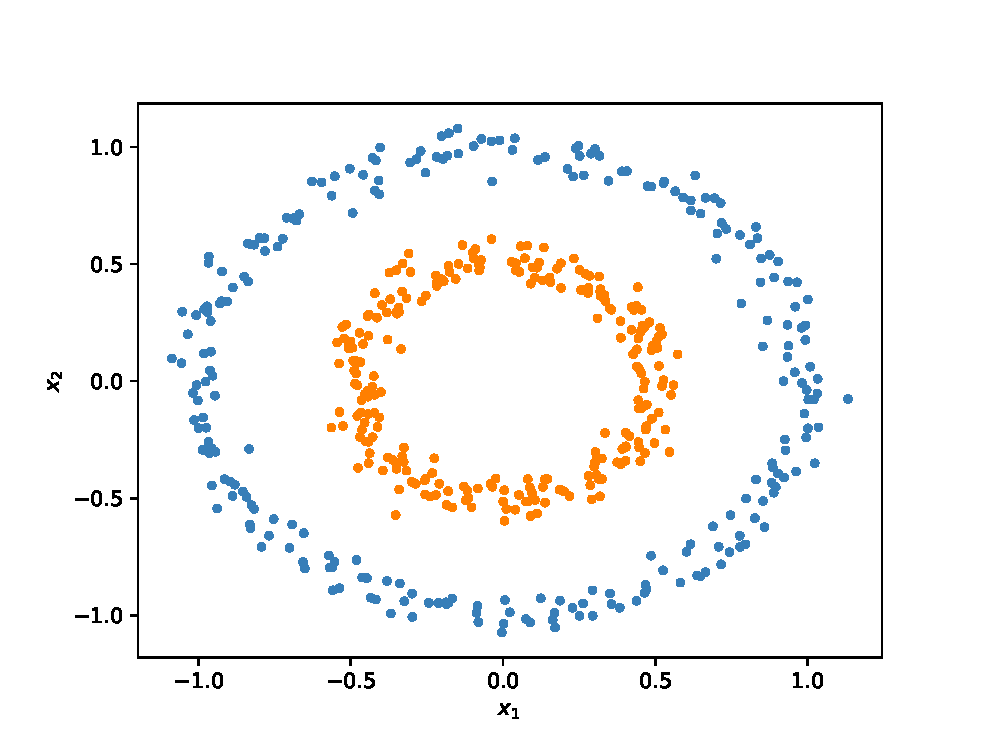
\includegraphics[height=0.5\textheight]{./figs/2d_poly_circle.eps}%
  \end{figure}
\end{frame}
%---------------------------------------------------------
\begin{frame}
  \frametitle{Lifting}
  One idea is to \textbf{LIFT} the samples into a higher dimensional space in which the samples are linearly separable.
  \begin{figure}
    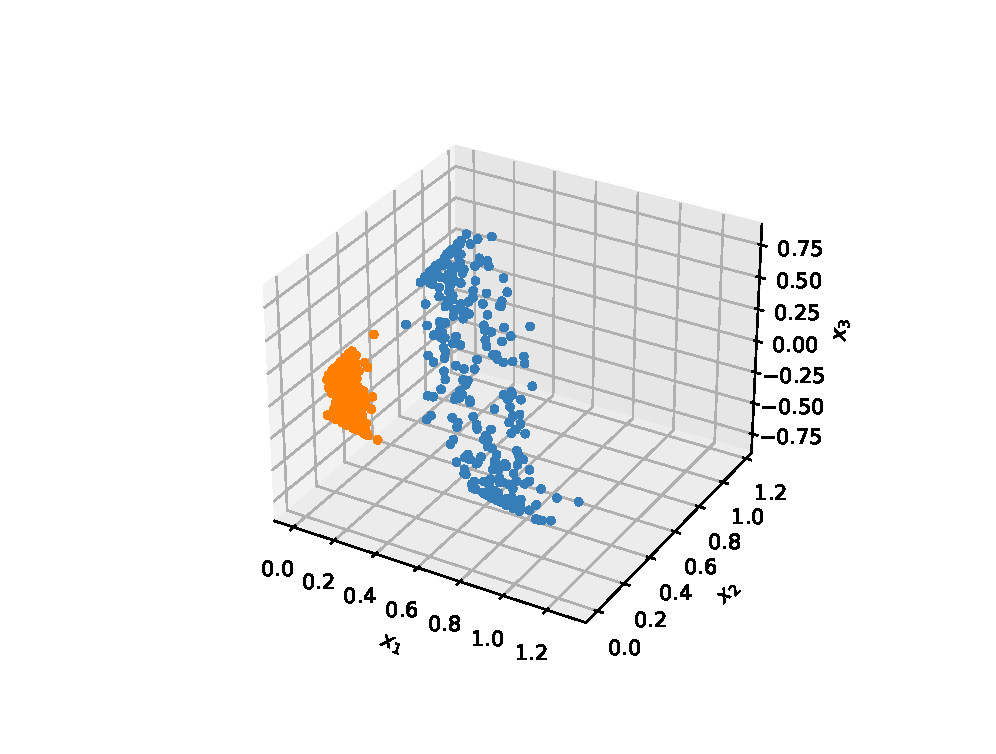
\includegraphics[height=0.45\textheight]{./figs/3d_poly_circle.eps}%
  \end{figure}
  The Lifting function in this case is 
  $
  \phi(X) = {
    \begin{bmatrix}
      x_{1,1}^2 \ x_{1,2}^2 \ \sqrt{2}x_{1,1}x_{1,2} \\
      x_{2,1}^2 \ x_{2,2}^2 \ \sqrt{2}x_{2,1}x_{2,2} \\
      \cdots \\
      x_{N,1}^2 \ x_{N,2}^2 \ \sqrt{2}x_{N,1}x_{N,2} 
    \end{bmatrix}
  }
  $.
\end{frame}
%---------------------------------------------------------
\begin{frame}
\frametitle{Curse of Dimensionality}
\begin{itemize}
  \item<1-> Consider solving the above problem with \emph{support vector machine} (SVM).
  \begin{align*}
    \mathcal{L}(\vec{w}, \vec{\alpha}) = \sum_{n=1}^N\alpha_n - \frac{1}{2}\sum_{n}^{N}\sum_{m}^{N}\alpha_n\alpha_m y_ny_m(x_n\trn x_m).
  \end{align*}
  The $\vec{w}$ is the linear decision boundary and $\vec{\alpha}$ is a vector of Lagrange multipliers.
  \item <2-> We need to use lifting function $\phi(X)$ to make the samples linearly separable. Specifically, we replace $(x_n\trn x_m)$ with $(\phi(x_n)\trn\phi(x_m))$.
  \begin{align*}
    \phi(x_n)\trn\phi(x_m) 
    &= \bracks*{x_{n,1}^2 \ x_{n,2}^2 \ \sqrt{2}x_{n,1}x_{n,2}}\bracks*{x_{m,1}^2 \ x_{m,2}^2 \ \sqrt{2}x_{m,1}x_{m,2}}\trn \\
    &= x_{n,1}^2x_{m,1}^2 + x_{n,2}^2x_{m,2}^2 + 2x_{n,1}x_{n,2}x_{m,1}x_{m,2}
  \end{align*}
  \item<3-> Calculate the inner product in the $\R^3$ across all $N$ pairs of samples is acceptable. However, the lifting function $\phi(X)$ is usually very high dimensional.
\end{itemize}
\end{frame}
%---------------------------------------------------------
\begin{frame}
  \frametitle{Kernel Trick}
  \begin{itemize}
    \item<1-> Consider the following derivation,
    \begin{align*}
      (x_n\trn x_m)^2 
      &= \parens*{\bracks*{x_{n,1} \ x_{n,2}}\bracks*{x_{m,1} \ x_{m,2}}\trn}^2 \\
      &= \parens*{x_{n,1}x_{m,1} + x_{n,2}x_{m,2}}^2 \\
      &= x_{n,1}^2x_{m,1}^2 + x_{n,2}^2x_{m,2}^2 + 2x_{n,1}x_{n,2}x_{m,1}x_{m,2} \\
      &= \phi(x_n)\trn\phi(x_m)
    \end{align*}
    \item<2-> Instead of computing inner product in the high dimensional space, we compute the inner product in the original space.
    \item<3-> The function 
    \begin{align*}
      K(x_n, x_m) = (x_n\trn x_m)^2 = \phi(x_n)\trn\phi(x_m)
    \end{align*}
     is called a \textbf{kernel function}.
  \end{itemize}
\end{frame}
%---------------------------------------------------------
\begin{frame}
  \frametitle{There must be disadvantages\ldots}
  \begin{itemize}
    \item<1-> Given training data $(x_1, y_1), (x_2, y_2), \ldots, (x_N, y_N) \in \mathcal{X}\times\mathcal{Y}$, where $\mathcal{X}\subseteq \R^d$ and $\mathcal{Y}\subseteq\R$. Consider \emph{Kernel Ridge Regression} (KRR), with $\phi(\mathcal{X})\subseteq \R^k$, where $k\rightarrow\infty$
    \begin{align*}
      \mathcal{L}(\vec{w}, \lambda)=\argmin_{\vec{w}}\sum_{n}^{N}(y_n - \vec{w}\trn\phi(\vec{x}_n))^2 + \lambda\vec{w}\trn\vec{w}.
    \end{align*}
    Solving it with Lagrange multipliers $\vec{\alpha}$, which is the solution of
    \begin{align*}%\label{}
      (\mathbf{K}+\lambda\mathbf{I}_k)\vec{\alpha} = \vec{y},
    \end{align*} 
    requires $\Theta(k^3)$ time and $\Theta(k^2)$ memory. Here $\mathbf{K}\in \R^{k\times k}$ is the kernel matrix or Gram matrix defined by $\mathbf{K}_{nm} \equiv K(\vec{x}_n, \vec{x}_m)$.
    \item<2-> \textbf{Intuition:} Can we find a kernel function which lifts $\mathcal{X}$ to $\R^s$, where $d < s\ll k$, while not sacrifices model performance?
  \end{itemize}
\end{frame}
%---------------------------------------------------------


\section{Random Fourier Features}
%---------------------------------------------------------
\begin{frame}
\frametitle{Some Prerequisites}
\begin{alertblock}{Shift Invariant Kernel (Radial Basis Kernel (RBK))}
  A kernel function $K(\vec{x_n}, \vec{x_m})$ is called \textbf{shift invariant} if it can be written as $K(\vec{x_n}, \vec{x_m}) = g(\vec{x_n}-\vec{x_m})$ for some function $g(\cdot)$
  
  (\eg $K_{Gaussian}(\vec{x_n},\vec{x_m})=\exp(-\gamma\norm{\vec{x_n}-\vec{x_m}}_2^2)$).
\end{alertblock}
\begin{block}{Mercer’s Theorem}
  A continuous function $K(\vec{x_n}, \vec{x_m})$ is a valid kernel function if and only if the kernel matrix $\mathbf{K}$ is \textbf{positive definite}.
\end{block}
\begin{block}{Bochner's Theorem}
  A continuous function $g(\cdot)$ is \textbf{positive definite} if and only if it is the Fourier transform of a non-negative measure.
\end{block}
\end{frame}
%---------------------------------------------------------
\begin{frame}
  \frametitle{Random Fourier Features}
  \begin{exampleblock}{Conclusion}
    A continuous \textbf{shift invariant} kernel $K(\vec{x_n}, \vec{x_m})$, which is \textbf{positive definite} (Mercer's Theorem), is the Fourier transform of a non-negative measure $p(\cdot)$.
    \begin{align}
      \phi(\vec{x_n})\trn\phi(\vec{x_m})
      &= K(\vec{x_n}, \vec{x_m}) = K(\vec{x_n}-\vec{x_m}) \\
      &=\int_{\R^s}p(\vec{\omega})\exp(i\vec{\omega}\trn(\vec{x_n}-\vec{x_m}))d\vec{\omega} \\
      &= \mathbb{E}_{\vec{\omega}}\bracks*{\xi(\vec{x_n})\xi(\vec{x_m})^*}\label{rffinC}
    \end{align}
    Here 
    $
    \xi(\vec{x})=\exp(i\vec{\omega}\trn\vec{x})={
      \begin{bmatrix}
        \cos(\vec{\omega}\trn\vec{x}) \\
        \sin(\vec{\omega}\trn\vec{x})
      \end{bmatrix}
    }
    $ 
    and hence $\xi(\vec{x_n})\xi(\vec{x_m})^*$ is an unbiased estimator of $K(\vec{x_n}, \vec{x_m})$.
  \end{exampleblock}
\end{frame}
%---------------------------------------------------------
\begin{frame}
  \frametitle{Algorithm}
  Since both the $p(\cdot)$ and $K(\triangle)$ are real-valued, we can replace $\xi(\vec{x})$ with $z_{\vec{\omega}}(\vec{x})=[\sqrt{2}\cos(\vec{\omega}\trn\vec{x}+b)]$ where $\vec{\omega}$ is drawn from $p(\vec{\omega})$ and $b$ is uniformly drawn from $[0, 2\pi]$. Then~\eqref{rffinC} becomes $\mathbb{E}_{\vec{\omega}}[z(\vec{x_n})z(\vec{x_m})\trn]$
  \begin{algorithm}[H]
    \caption{An algorithm with caption}\label{alg:cap}
    \begin{algorithmic}[1]
    \Require $n \geq 0$
    \Ensure $y = x^n$
    \State $y \gets 1$
    \State $X \gets x$
    \State $N \gets n$
    \While{$N \neq 0$}
    \If{$N$ is even}
        \State $X \gets X \times X$
        \State $N \gets \frac{N}{2}$  \Comment{This is a comment}
    \ElsIf{$N$ is odd}
        \State $y \gets y \times X$
        \State $N \gets N - 1$
    \EndIf
    \EndWhile
    \end{algorithmic}
  \end{algorithm}
\end{frame}
%---------------------------------------------------------


%---------------------------------------------------------
%Two columns
\begin{frame}
\frametitle{Two-column slide}
\framesubtitle{This is a subtitle}

\begin{columns}

\column{0.5\textwidth}
This is a text in first column.
\begin{align*}
  E=mc^2
\end{align*}
\begin{itemize}
\item First item $\ell$
\item Second item
\end{itemize}

\column{0.5\textwidth}
This text will be in the second column
and on a second thought this is a nice looking
layout in some cases.
\end{columns}
\end{frame}
%---------------------------------------------------------


\end{document}